
% Operations Manual Title
\infolevone{
\section{M\o ller Polarimeter }
%\setcounter{subsection}{0}

The M\o ller Polarimeter is used to measure the electron beam
polarization. Instructions for carrying out such a measurement
are documented in a 
\htmladdnormallinkfoot{Step-by-Step Guide}{http://www.jlab.org/Hall-C/document}.
MCC follows a complementary 
\htmladdnormallink{procedure}{http://opsntsrv.acc.jlab.org/ops_docs/online_document_files/MCC_online_files/HallC_Moller_pol_measurement_proc.pdf}.
The polarimeter is located at the end of the Hall C alcove downstream
of the Compton polarimeter.  All magnetic elements of the polarimeter
are located between the BPMs 3C21 and 3H02: there are a solenoid and
three quadrupoles.  The M\o ller target is located in the center of
the solenoid. The detectors are positioned 11 meters downstream of the
target and 0.49 meters away from the beam line in a lead house.

The Hall~C M\o ller polarimeter consists of: the target and target
solenoid, the quadrupole magnets, a collimator box, and the detectors.
These are described in turn in the paragraphs below:

{\sl Target Solenoid} This is a $\approx$ 4 T super conducting
solenoid used to ``brute force" polarize the valence electrons in a
thin, $\approx$ 4 $\mu$m, iron foil perpendicular to the plane of the
foil. This magnet has a liquid nitrogen cooled radiation shield and
requires liquid helium for operation.

{\sl Quadrupole Magnets} In order to keep the locations of the M\o
ller target and detectors fixed regardless of the incident beam energy
a ``two'' quadrupole optics was chosen. The first quadrupole (the
``Los Alamos'' or small M\o ller quad) has a 4 inch bore and a
physical length of about 1 ft.  The second focusing element is
actually a pair of identical quadrupoles (10Q36, large M\o ller quads)
each with a 10 inch bore and physical length of 123 cm. The
quadrupoles are wired in series and operated as one magnet for use at
high energies.

{\sl Collimator Box} There are seven movable blocks of densimet
(densimet is a machinable alloy of tungsten) for the collimator. These
blocks form two horizontal jaw pairs and one vertical jaw pair. The
seventh block has a hole in it through which the unscattered electron
beam travels.

{\sl Detectors} The Hall~C polarimeter was built to operate in
coincidence mode with both the scattered and recoiling electrons being
detected in coincidence. There are thus two identical detector stacks
placed symmetrically about the beamline. Each stack consists of a
sixteen element hodoscope followed by a lead glass block.

\paragraph{Polarimeter Description}
The layout of the polarimeter is shown in fig.~\ref{fig:polsketch}.
The incoming electron beam hits an iron target foil. The target
thickness is on the order of 1 to 10 $\mu m$. The electrons in the
iron foil are polarized by the 3-4 T magnetic field of the super
conducting solenoid.  The beam electrons scatter off the target
electrons (M\o ller Scattering) with the scattering angle of interest
at about 1$^{\circ}$ or below in the laboratory system. Since the
electrons are very close to the beam line they need to be deflected
away from it in order to be detected in coincidence. This is achieved
by the quadrupoles. The first smaller quadrupole is focusing in the
horizontal plane while the second and third large quadrupoles
defocusing in the same plane. The use of two (three) quadrupoles
allows us to keep the cone of the 90$^{\circ}$ CM scattered electrons
at fixed dimensions after a 11 meter drift distance.  In the 6 GeV
era, only one large quadrupole was used, the size of the 90 degree
cone was 49~cm horizontal and 16~cm vertical from the beam line. This
tune can still be used (if only one large quad is used) up to a beam
energy of about 5~GeV. In the new configuration (with two large
quads), the cone of the CM scattered electrons is 49~cm and 9~cm
vertical from the beamline. This option can be used over the full
range of available beam energies, up to 11 GeV.

The first quadrupole (the Los Alamos quad) has a 4 inch bore and a
physical length of 12 inches. The second pair of quadrupoles (10Q36)
has a 10 inch bore and a physical length of 123 cm.
\begin{figure}[htp]
\begin{center}
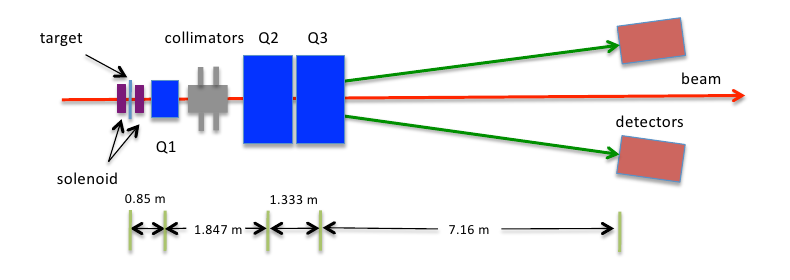
\includegraphics[width=6in]{moller_layout_12gev.png}
\caption{Sketch of the M\o ller polarimeter in Hall C.\label{fig:polsketch}}
\end{center}
\end{figure}
The two electrons are detected in coincidence using two lead glass
shower counters as shown in Figure \ref{detarr}. In front of each
counter is a collimator that defines the acceptance. The right
collimator is intentionally larger than the left. This reduces the
sensitivity of the coincidence acceptance to beam and detector
positions. In front of the collimator is a hodoscope with 16
channels. Each channel is a scintillator of 1cm width.
\begin{figure}
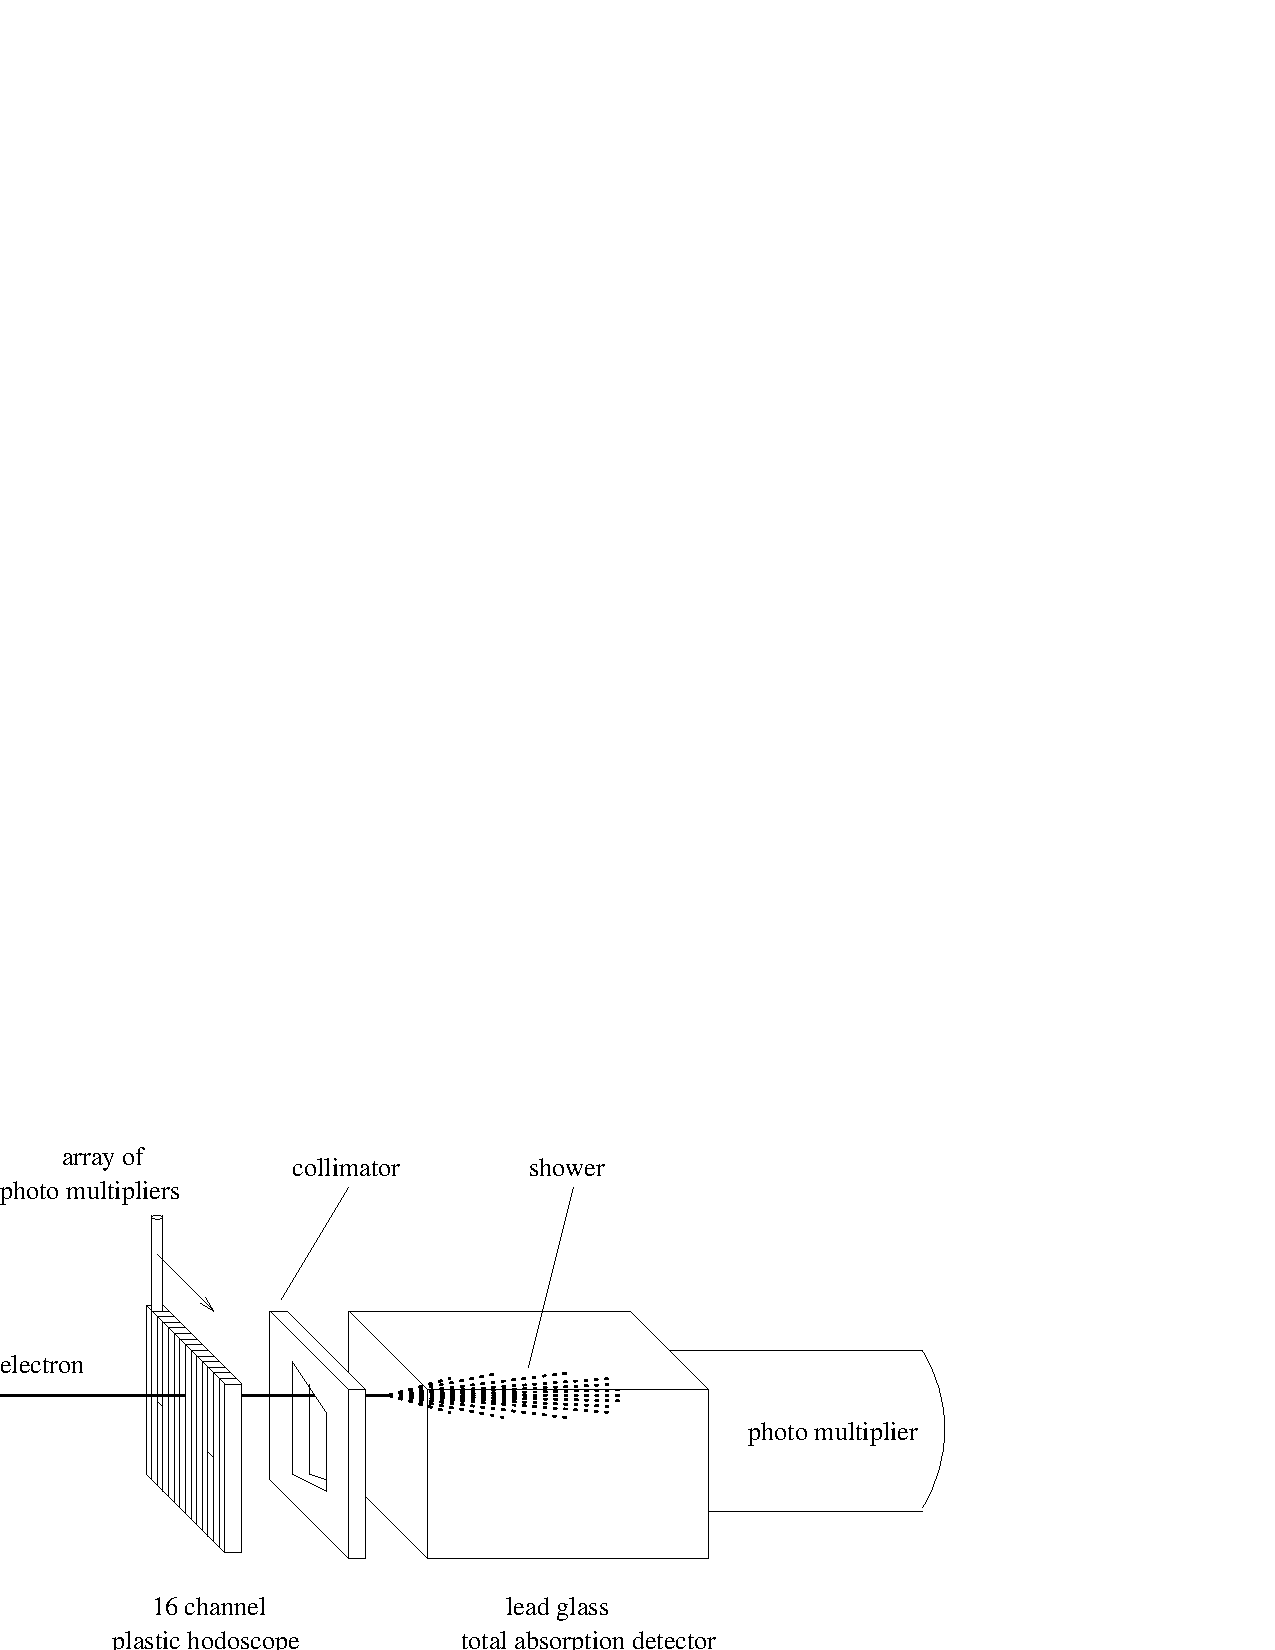
\includegraphics[width=6in]{detarangement.pdf}
\begin{center}
\parbox{10cm}{
\caption{Detector arrangement}\label{detarr}}
\end{center}
\end{figure}

Since the cross section for Mott scattering (electron - nucleus
scattering) is much larger than M\o ller scattering it is necessary to
use collimators to reduce this background that leads to accidental
coincidences. This is achieved with a set of movable collimators
located between the small and large quadrupoles (see
fig.~\ref{fig:polsketch} and \ref{colscetch}).
%
\begin{figure}[htb]
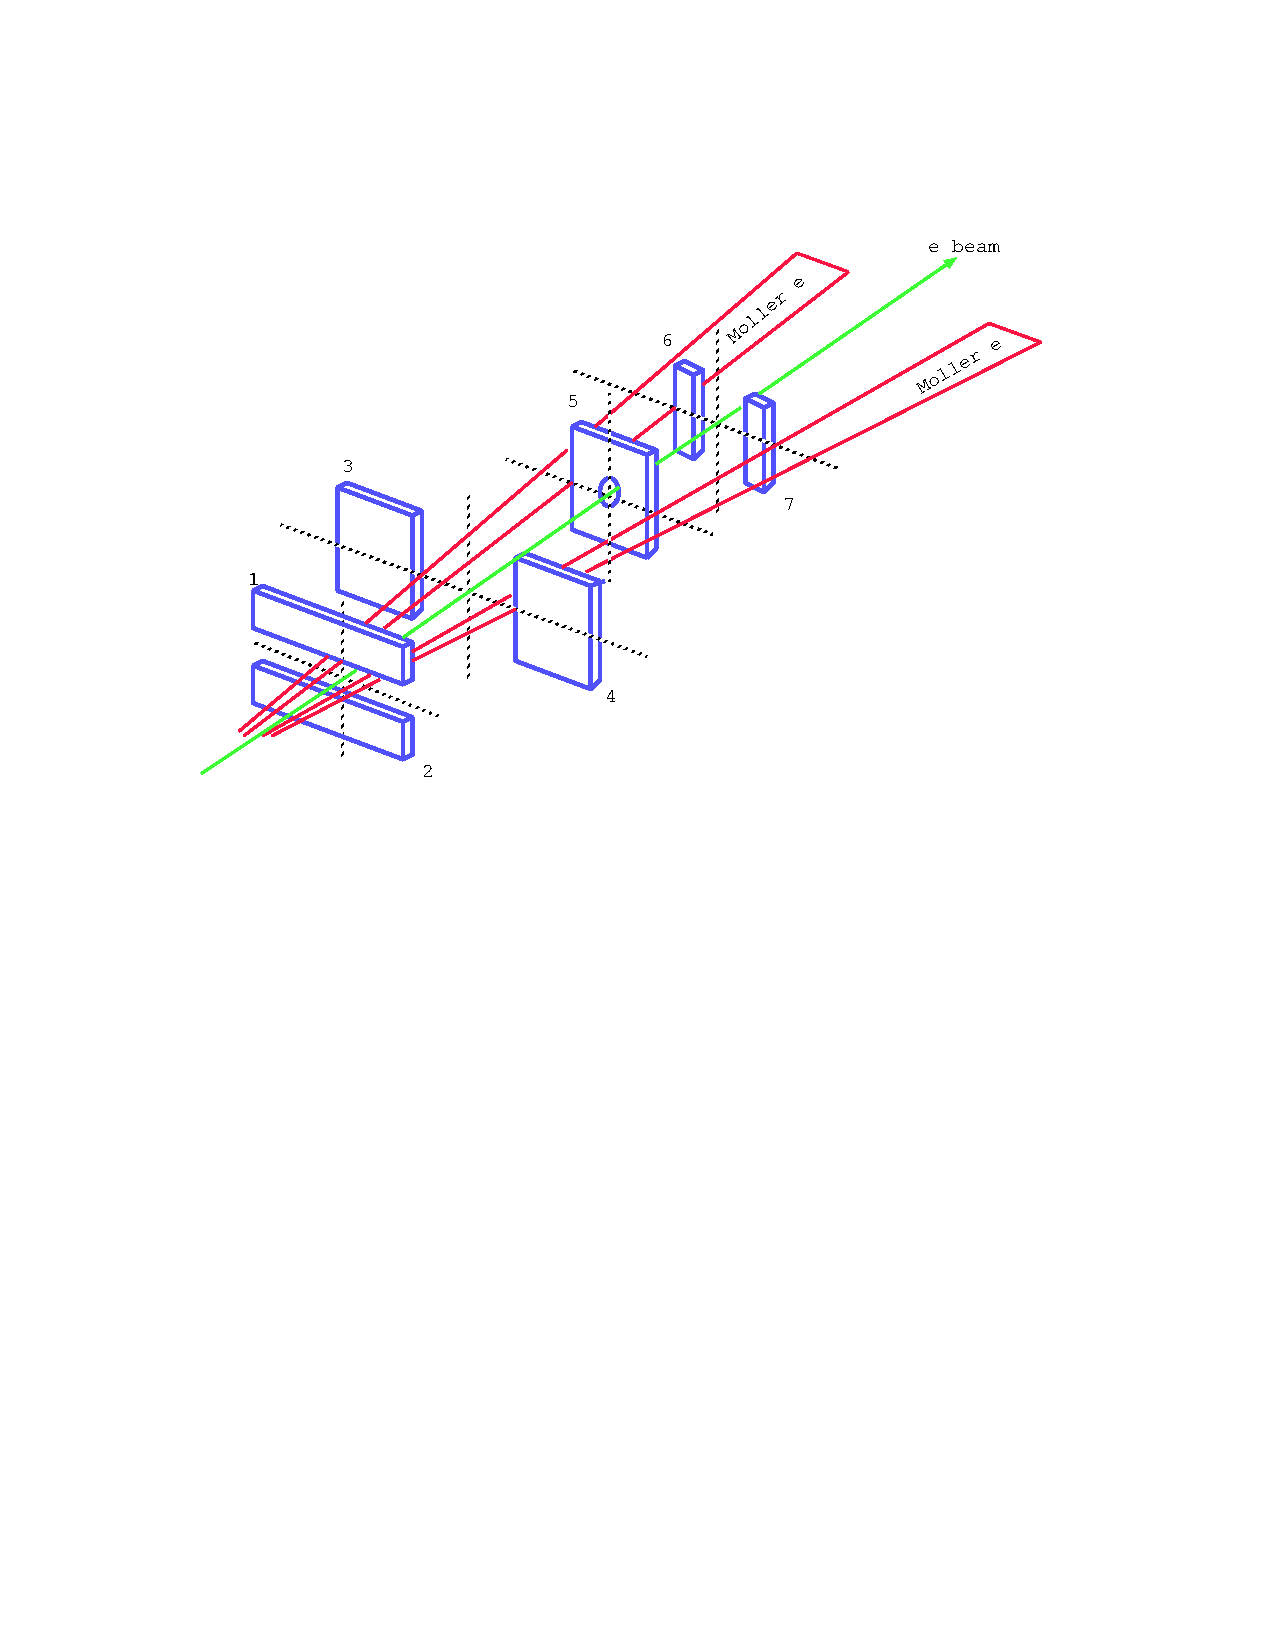
\includegraphics[width=15cm]{collim.pdf}
\begin{center}
\caption{Collimator with M\o ller trajectories\label{colscetch}}
\end{center}
\end{figure}
Mott electrons with the right momentum and scattering angle that make
it through the quadrupoles into the detectors do not follow the same
path in configuration space as the M\o ller electrons do.  The
collimators are used to shield the space that is not traversed by the
M\o ller electrons. The space of the M\o ller stripes is given by the
collimators in front of the lead glass detectors that define the
coincidence acceptance.
%

\paragraph{M\o ller Control Software and Hardware}
There are three main control packages for the M\o ller Polarimeter.
Two of them are GUIs run from the Hall C Counting Room. They control
1)~the solenoid cryogenics, and 2)~the solenoid field, the target, and
the collimators. Control of the M\o ller quadrupoles is possible only
from MCC, although the second counting room GUI does allow
experimenters to monitor the quadrupole settings.


\begin{figure}[htb]
  \begin{center}
%  \htmlimage{scale=1.0,thumbnail=0.5}
  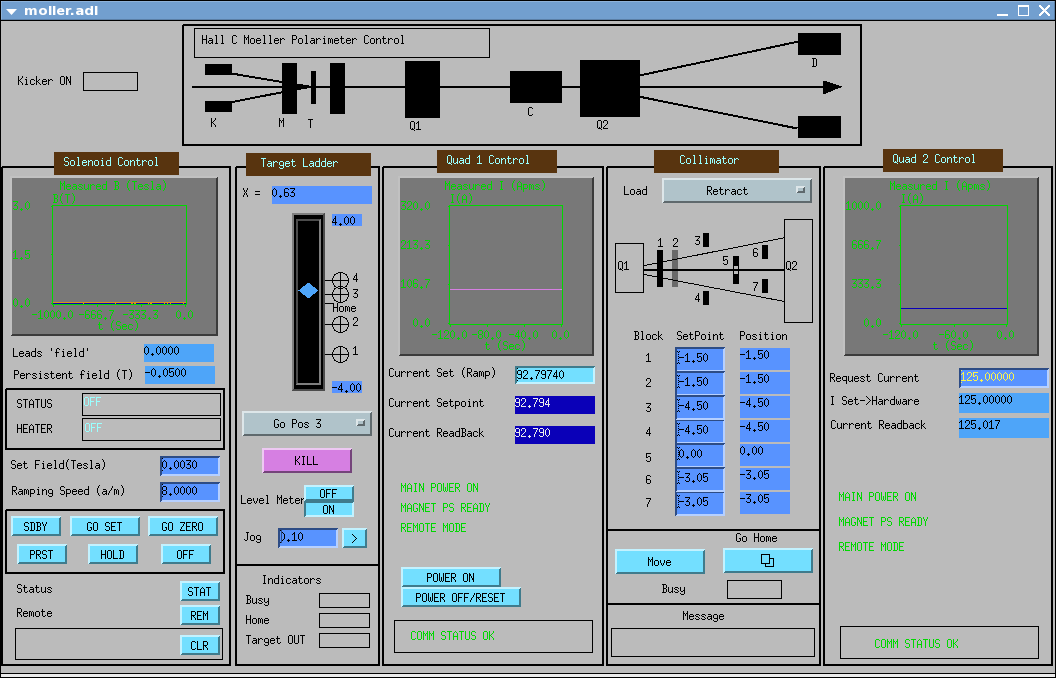
\includegraphics[width=15cm]{moller_controls.png}
  \caption{M\o ller Polarimeter Control GUI\label{molpolmedm}}
  \end{center}
\end{figure}
%

\subparagraph{Polarimeter GUI}

To run the GUI using medm do the following steps
\begin{itemize}
\item Log onto to any cdaqlX machine from the account \texttt{cvxwrks}.
\item Set directory: \texttt{cd \textasciitilde{}/MEDM/moller}
\item Start the GUI: \texttt{medm moller.adl}
\end{itemize}
%

\subparagraph{Quadrupole Settings}

Although the quadrupoles are controlled only by MCC, it is the
responsibility of the experimenter to make certain that they are set
to the correct currents. The correct currents are a function of the
incident beam energy .  The initial settings are determined by a
simple optics model of the M\o ller polarimeter and the final values
are determined empirically by tuning the system using beam. The final
currents are determined experimentally by optimizing the M\o ller
hodoscope left-right correlation. This guarantees that the polarimeter
acceptance is centered around 90 degrees in the center of mass.
Predicted quadrupole currents for several beam energies are shown in
Tab.~\ref{tab_qcurrent}.

%
% Old - from 6 GeV setup. No longer accurate.
%\begin{table}[!hbt]
%\begin{center}
%\begin{tabular}{|c|c|c|l|} \hline
%Beam Energy & Q1  & Q2 &Reference data \\
%\hline
%0.884 &  85.9 & 112.0 & March, 2001  \\
%2.332 & 136.0 & 364.0 & August, 2001 \\
%2.415 & 137.1 & 380.0 & April, 2001  \\
%3.395 & 142.2 & 586.0 & March, 2001  \\
%\hline 
%\end{tabular}
%\caption{M\o ller Quadrupole Current Settings\label{tab_qcurrent}}
%\end{center}
%\end{table}

\begin{table}[!hbt]
\begin{center}
\begin{tabular}{|c|c|c|} \hline
Beam Energy (GeV) & Q1 (A)  & Q2/Q3 (A) \\
\hline
1.0 &  102.14 & 60.85 \\
5.0 & 159.73 & 423.18 \\
9.0 & 114.13  & 937.85 \\
11.0 & 100.10 & 1352.24 \\
\hline 
\end{tabular}
\caption{M\o ller Quadrupole Current Settings from optics model predictions.\label{tab_qcurrent}}
\end{center}
\end{table}

%A reminder to the expert: After a power failure or power cycle of the Q1 
%power supply and/or controller,
%it is necessary to press the green "START" button on the Q1 (Small
%M\o ller Quad) power supply.  If MCC cannot get any real current out of the
%supply then probably it is in standby mode and needs the START button pushed.

Currently the Degauss procedure for Q2 and Q3 is to ramp the magnet up
to 800 Amps then ramp down to zero, reverse polarity, ramp to -240 Amp
and finally back to zero. This procedure is almost never used and is
not known to be important.

%
\subparagraph{Target Motion}
There are four possible target positions, shown in
Table \ref{tab_moltar}. They can be selected using the GUI with the
frame title {\tt ``Target Ladder''} . In the menu indicated by the
term {\tt ``Cancel''} the four individual target positions can be
selected. Once chosen with the mouse pointer the target ladder will
move! {\bf ALWAYS (BEAM OFF) WHEN TARGET IS BEING MOVED.}  Since the
target positions are hardwired in the code, any corrections to these
values need to be done manually using the {\tt ``Jog''} option of the
GUI. The camera button {\tt ``ON OFF'' } turns the target camera and
light on and off respectively.

\begin{table}
\begin{center}
\begin{tabular}{|c|c|c|l|} \hline
Target & Material & Thick $\mu$m & Position \\
\hline
1 & Fe & 1 & -2.03   \\
2 & Fe & 4 & -0.56  \\
3 & Fe & 1 & +0.93  \\
4 & Empty & - & N/A    \\
\hline 
\end{tabular}
\parbox{10cm}{
\caption{M\o ller Targets\label{tab_moltar}}}
\end{center}
\end{table}
%
After a power cycle the target first needs to find HOME. This can be
done selecting the {\tt ``HOME''} in the menu. To move the target
ladder fully out of the beam select {\tt ``RETRACT''} from the menu.
At position -3.86 the target is fully out of the beam.
%
\subparagraph{Collimator Positions}
{\bf Never move collimator 5 while beam is present!!!}\\ {\bf Never
issue the Go Home while beam is present!!!}\\ The collimator positions
also depend on beam energy. However this dependency is only small
since the collimators do not need to be located very tight to the M\o
ller stripes. The singles rates do not increase significantly if the
collimators are even 5 mm away from the M\o ller stripes. The starting
values for the M\o ller collimators can be determined using the M\o
ller Monte Carlo.

Each collimator can be moved individually be typing a value in the
column {\tt ``SetPoint''} at the appropriate window, see
fig. \ref{molpolmedm}. Use the {\tt ``RETURN''} key to set the value
and the {\tt ``Move''} button to move the collimator to this
value. For the collimators 1,2,3,4,6 the values can not be larger than
zero because that would move the collimators into the beam (software
cut). The collimator 5 is a special case since the beam goes through a
central hole in the collimator.  After a power cycle all the
collimators need to find the HOME position first.  This is done by
using the {\tt ``Go Home''} menu that pops up a window to ask if one
really want to search the home position.
%
\subparagraph{Target Solenoid}
Since the target solenoid is superconducting and therefore cooled with
liquid helium the controls are somewhat more complicated.  Currently
we run the magnet at a field of 3.5 Tesla. Before ramping up the
magnet, check the helium and nitrogen levels (see
Fig. \ref{molcryomedm}). The magnet has to be put into standby mode
first, this turns the heater on.  Use button {\tt ``SDBY''}.  After 20
seconds one can ramp up the magnet using the {\tt ``GO SET''} button.
This ramps up the magnet to the field value set in the frame {\tt
``Set Field(Tesla)''}.  After reaching the desired field the magnet
can be put into persistent mode (i.e. turns off the heater) by hitting
the button {\tt ``PRST''}.  If the solenoid will not be left at full
field for a significant period of time (more than several hours), it
is not necessary to put the magnet in persistent mode.  The maximum
ramp up speed is 12 Amps per minute.
%However, the first ramp-up after a thermal cycle should be made at
%6~amps/minute up to 2.4~T, followed by 3~amps/minute to 3~T.
The power supply has an internal ramp up parameter
that will limit ramping to 4 Amps per minute at higher fields.
The ramp up process can be stopped at any time by hitting the {\tt
``HOLD''} button. \\ \\
After a power cycle the remote button {\tt ``REM''} has to be activated
first in order to establish communication to the power supply.
The power supply is an IPS120-10 from OXFORD. Since it is a polarity
reversible device the sign of the field value chosen by the
{\tt ``Set Field(Tesla)''} is important. To reverse polarity the magnet
needs to be ramped down to zero first.
%

\subparagraph{M\o ller Cryogenics GUI}
The liquid nitrogen and helium supplies are monitored and controlled
by a GUI with the drivers running on the IOC vmec10 (aka {\it
iochc10}).  A screen snapshot is shown in Figure \ref{molcryomedm}.
To run the GUI using medm, perform the following steps:
\begin{itemize}
\item Log onto to any cdaqlX machine from the account \texttt{cvxwrks}.
\item Set directory: \texttt{cd MEDM/Moller/CRYO}
\item Start the GUI: \texttt{medme hcmcryo.adl}
\end{itemize}

\begin{figure}[htb]
\begin{center}
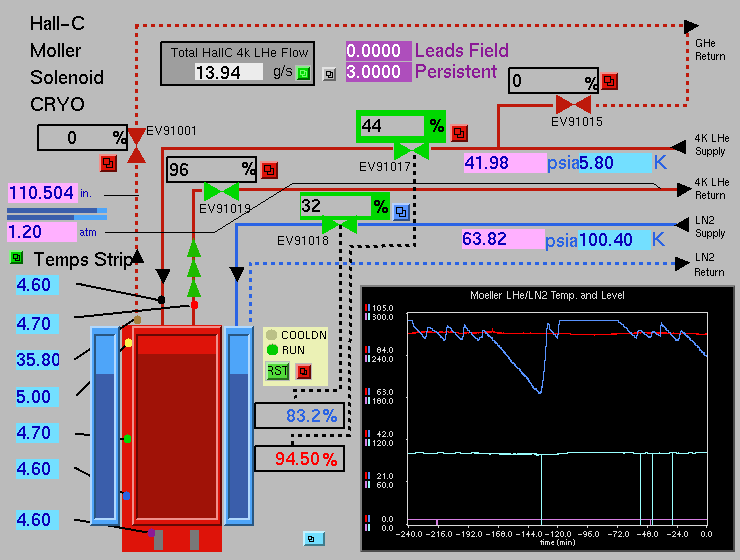
\includegraphics[width=15cm]{moller_cryo.png}
\caption{M\o ller Cryo GUI\label{molcryomedm}}
\end{center}
\end{figure}
%

Normally, the cryogen levels in the solenoid cryostat should be
automatically maintained at or above 60\% by the controls software.
If mandated, you may turn off the supply of helium or nitrogen by
closing JT-valves {\tt EV91017} or {\tt EV91018}, respectively.

Note that if VMEC10 (iochc10) gets rebooted, it is necessary to
RESTORE the cryo valve parameters for the M\o ller. You do this by
clicking on the small blue box on the bottom of the cryo overview
screen (hcmcryo.adl), selecting "SAVE/RESTORE", then selecting
"iochc10:NORMAL RESTORE" from the "!" box in the resulting screen. It
will prompt you to hit ENTER several times. Do so until the dialog
window goes away.

Cooling down the magnet from room temperature should only be done by a
M\o ller cryo expert in coordination with the JLab Cryo group. In
general, the steps are:
\begin{enumerate}
  \item{Make sure all all supply valves and the helium cold
        return valve are closed and the warm return is
        open.}
  \item{Open the LN2 supply valve (EV91017) and allow
        the transfer line and cryostat to cool down.  When the
        nitrogen reservoir is full, turn on the supply valve PID
        loop.}
  \item{Pre-cool the M\o ller cold return line by
        flowing cold helium backwards through the cold return to the
        warm return (EV91001) by opening the cold return valve
        (EV91019).}
  \item{Close the cold return and start cooling the
        helium transfer line helium reservoir by opening
        EV91017}
  \item{Once the helium reservoir is full, gradually
        open the cold return - once it is fully open, start closing
        the warm return.}
  \item{Once the warm return valve is closed,
        the helium valve control PID loops should be engaged
        (Figs.~\ref{fig:ev17c},\ref{fig:ev17c},
        and \ref{fig:ev17stc}).}
\end{enumerate}     
%The steps are
%\begin{enumerate}
%	\item Close {\tt EV91019} to isolate the cold return line.
%	\item Open {\tt EV91018} to about 35\% and flow nitrogen at this rate
%		until the nitrogen level indicator shows liquid in the cryostat.
%		This may take several hours. (You may start precooling the helium
%		lines [below] at the same time.)
%	\item Using the submenu pushbutton for {\tt EV91018}, put the valve on
%		PID control. PID parameters should be:
%	\begin{enumerate}
%		\item Max Pos = 35.0
%		\item Min Pos = 7.0
%		\item Max Chg = 15.0
%		\item Min CHg = 0.1
%		\item Set Val = 90.0
%		\item ST = 60.0
%		\item Gp = 1.0
%		\item Gi = 0.025
%		\item Gd = 0.0
%	\end{enumerate}
%	\item Observe that the nitrogen level now controls the position of {\tt EV91018}.
%	\item pre-cool the helium lines by opening {\tt EV91001} to 100\% and
%		opening {\tt EV91017} as much as possible without exceeding the total
%		Hall-C 4K helium consumption limit. Monitor the flow and 
%		reduce {\tt EV91017} as the system cools down (the flow will 
%		increase as the system temperature nears 4K).
%	\item When the cryostat helium level indicator shows 50\% or higher, put
%		{\tt EV91017} on automatic control. The supply JT valve is controlled 
%		such that both the liquid level and the supply temperature are maintained
%		at reasonable values. The standard PID parameters are shown in 
%		figs.~\ref{fig:ev17c}, \ref{fig:ev17llc} and~\ref{fig:ev17stc}.
%	\item The system is now in automatic control with {\it Warm Return}. Normally it
%		runs in {\it Cold Return}, which is much more energy efficient. Procedures
%		for transitioning to {\it Cold Return} will be forthcoming. Until they
%		are approved for non-expert use, contact Paul Brindza to switch the
%		system to {\it Cold Return}.
%\end{enumerate}

\begin{figure}[h!]
\centering
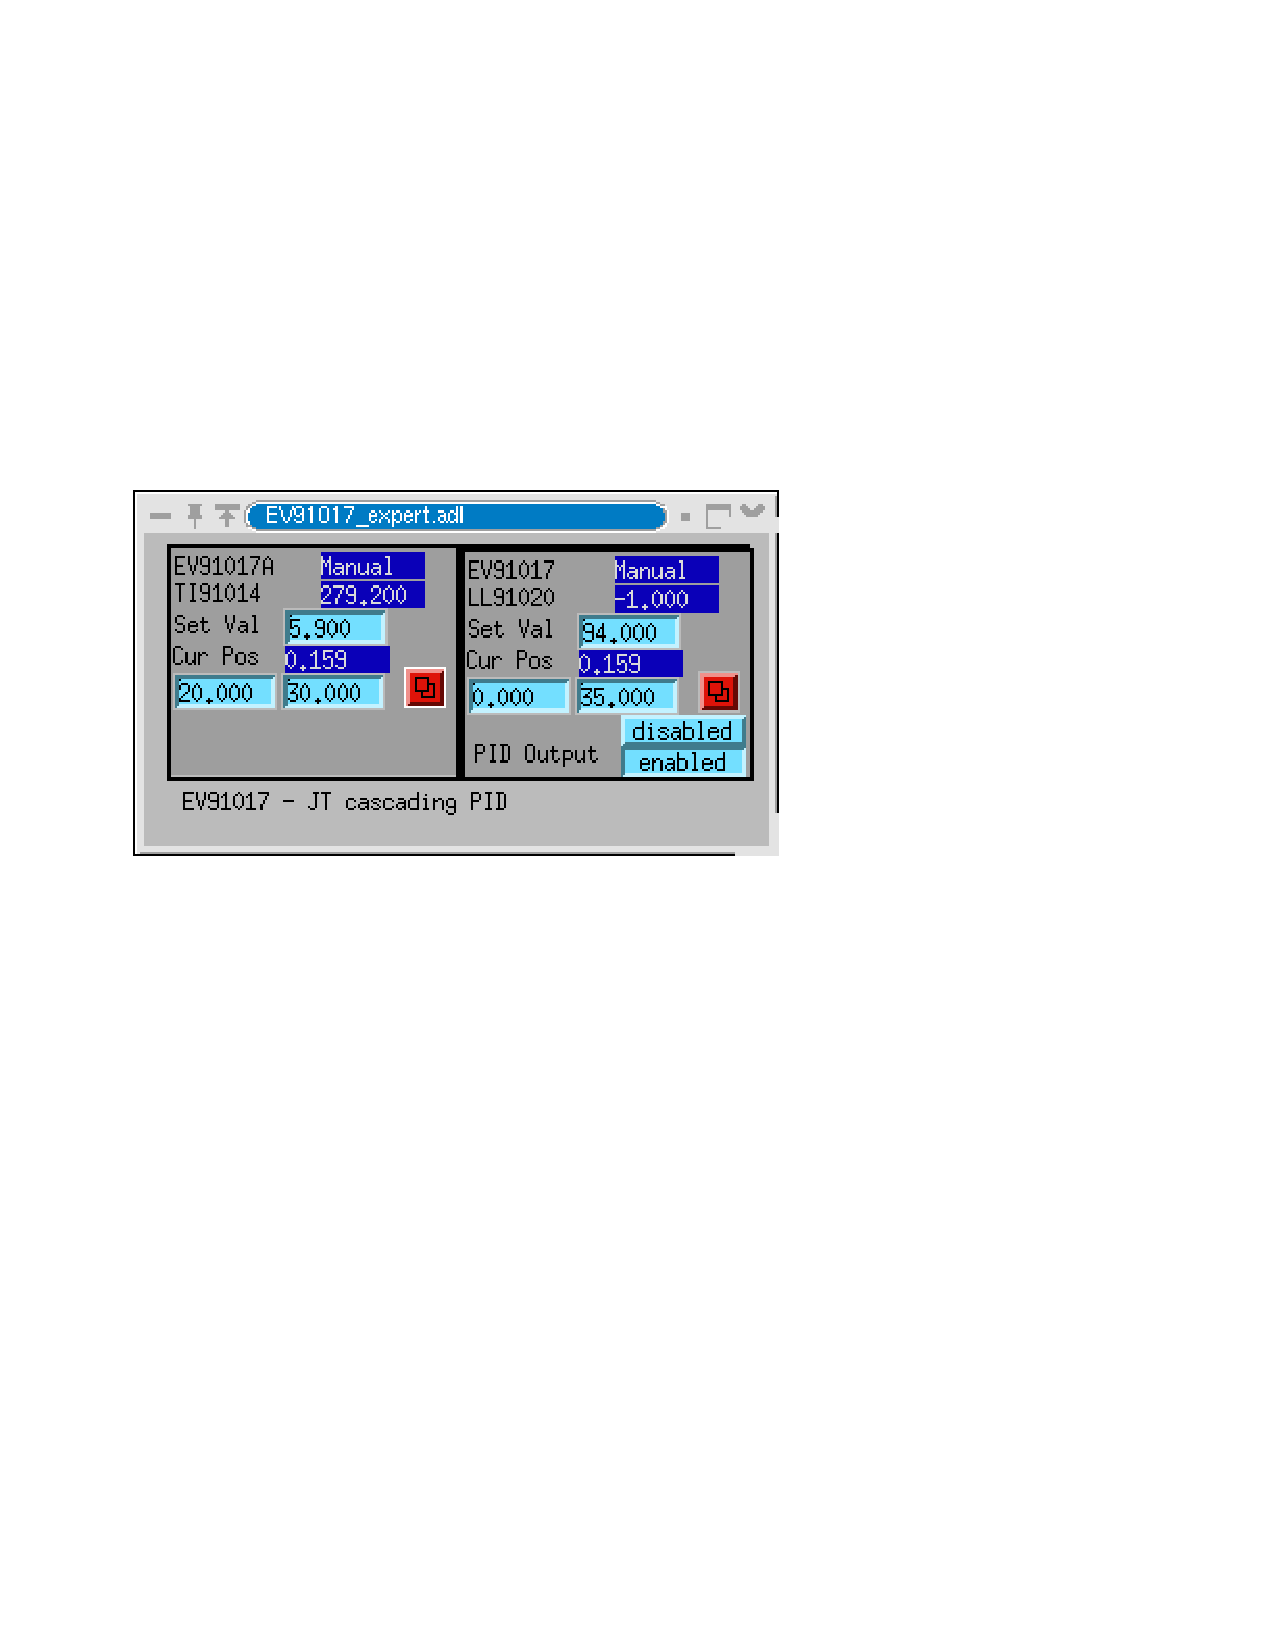
\includegraphics[width=3in]{ev91017_cascade.pdf}
\caption{PID MEDM Screen - EV91017 Cascade Loop}
\label{fig:ev17c}
%----------------------------
\end{figure}


\begin{figure}[h!]
\centering
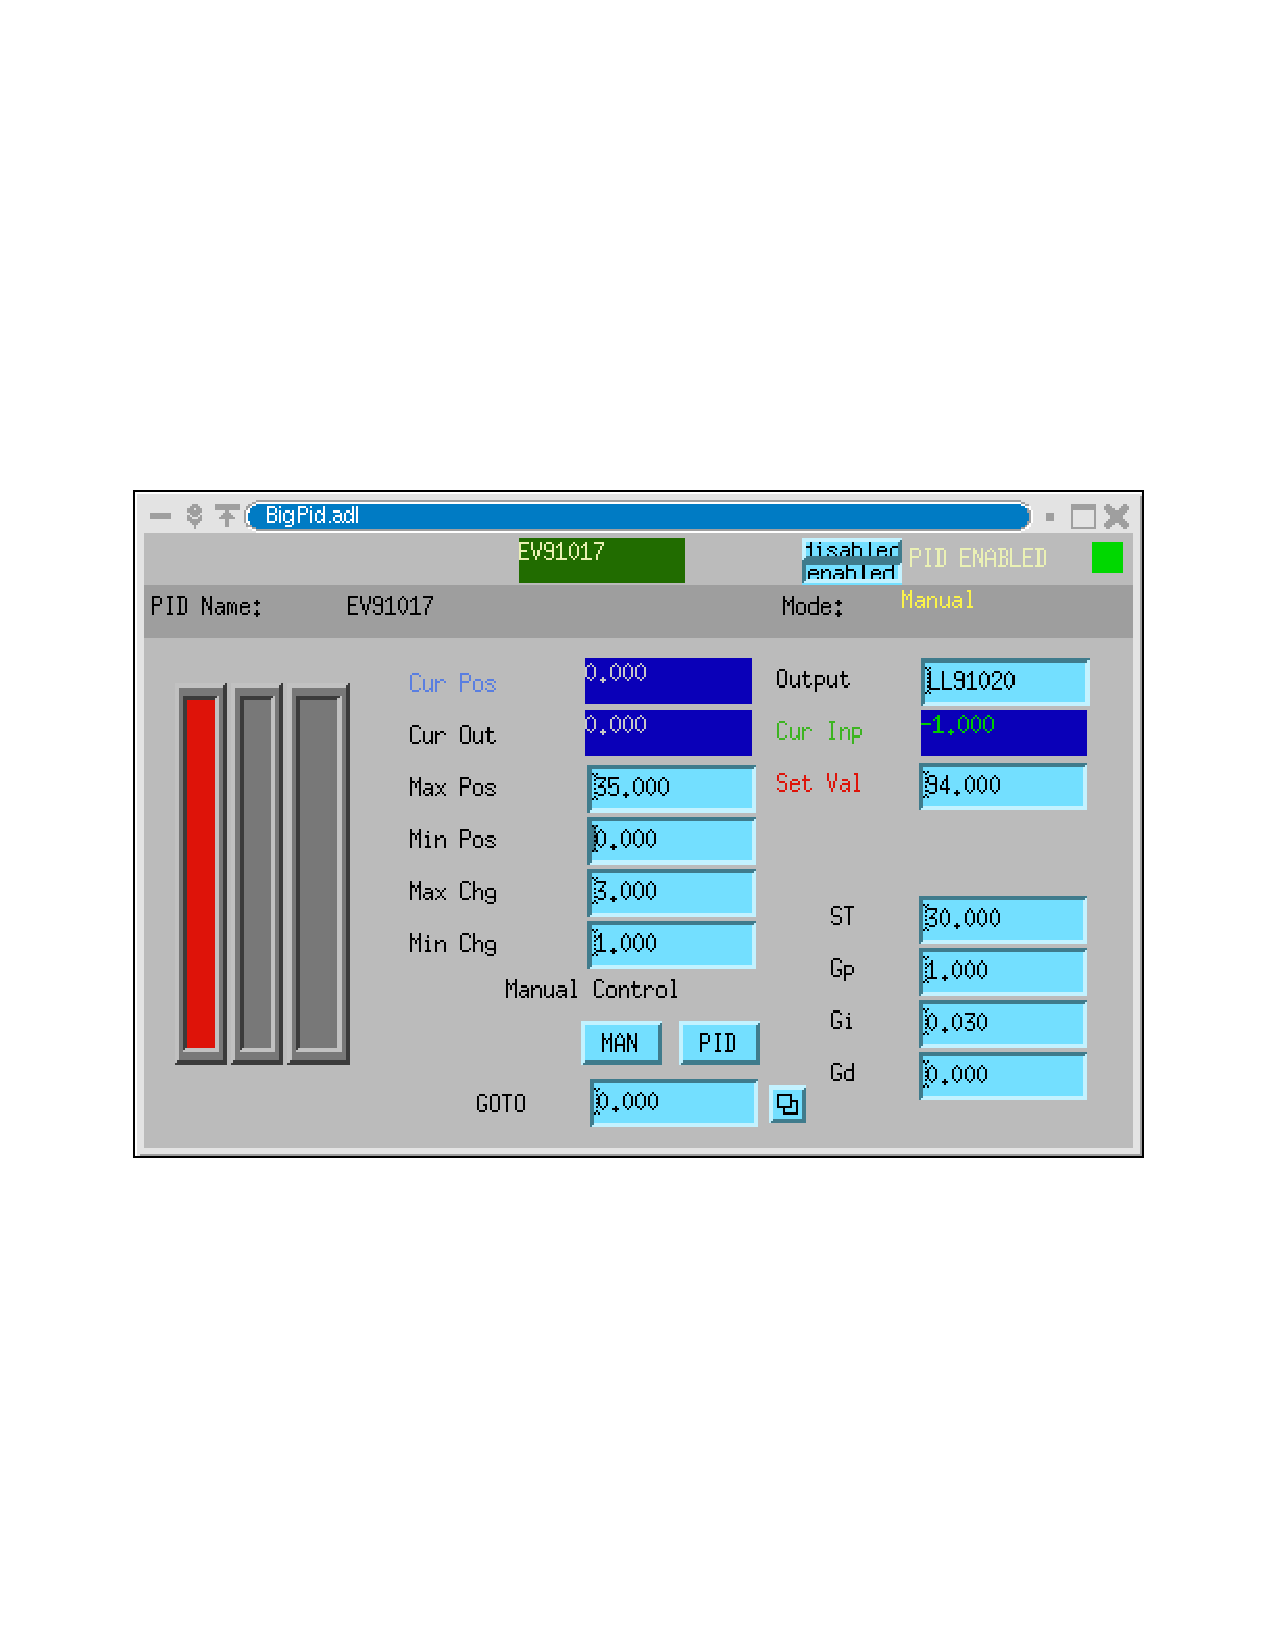
\includegraphics[width=3in]{ev91017.pdf}
\caption{PID MEDM Screen - EV91017 Liquid Level Control}
\label{fig:ev17llc}
\end{figure}


\begin{figure}[h!]
\centering
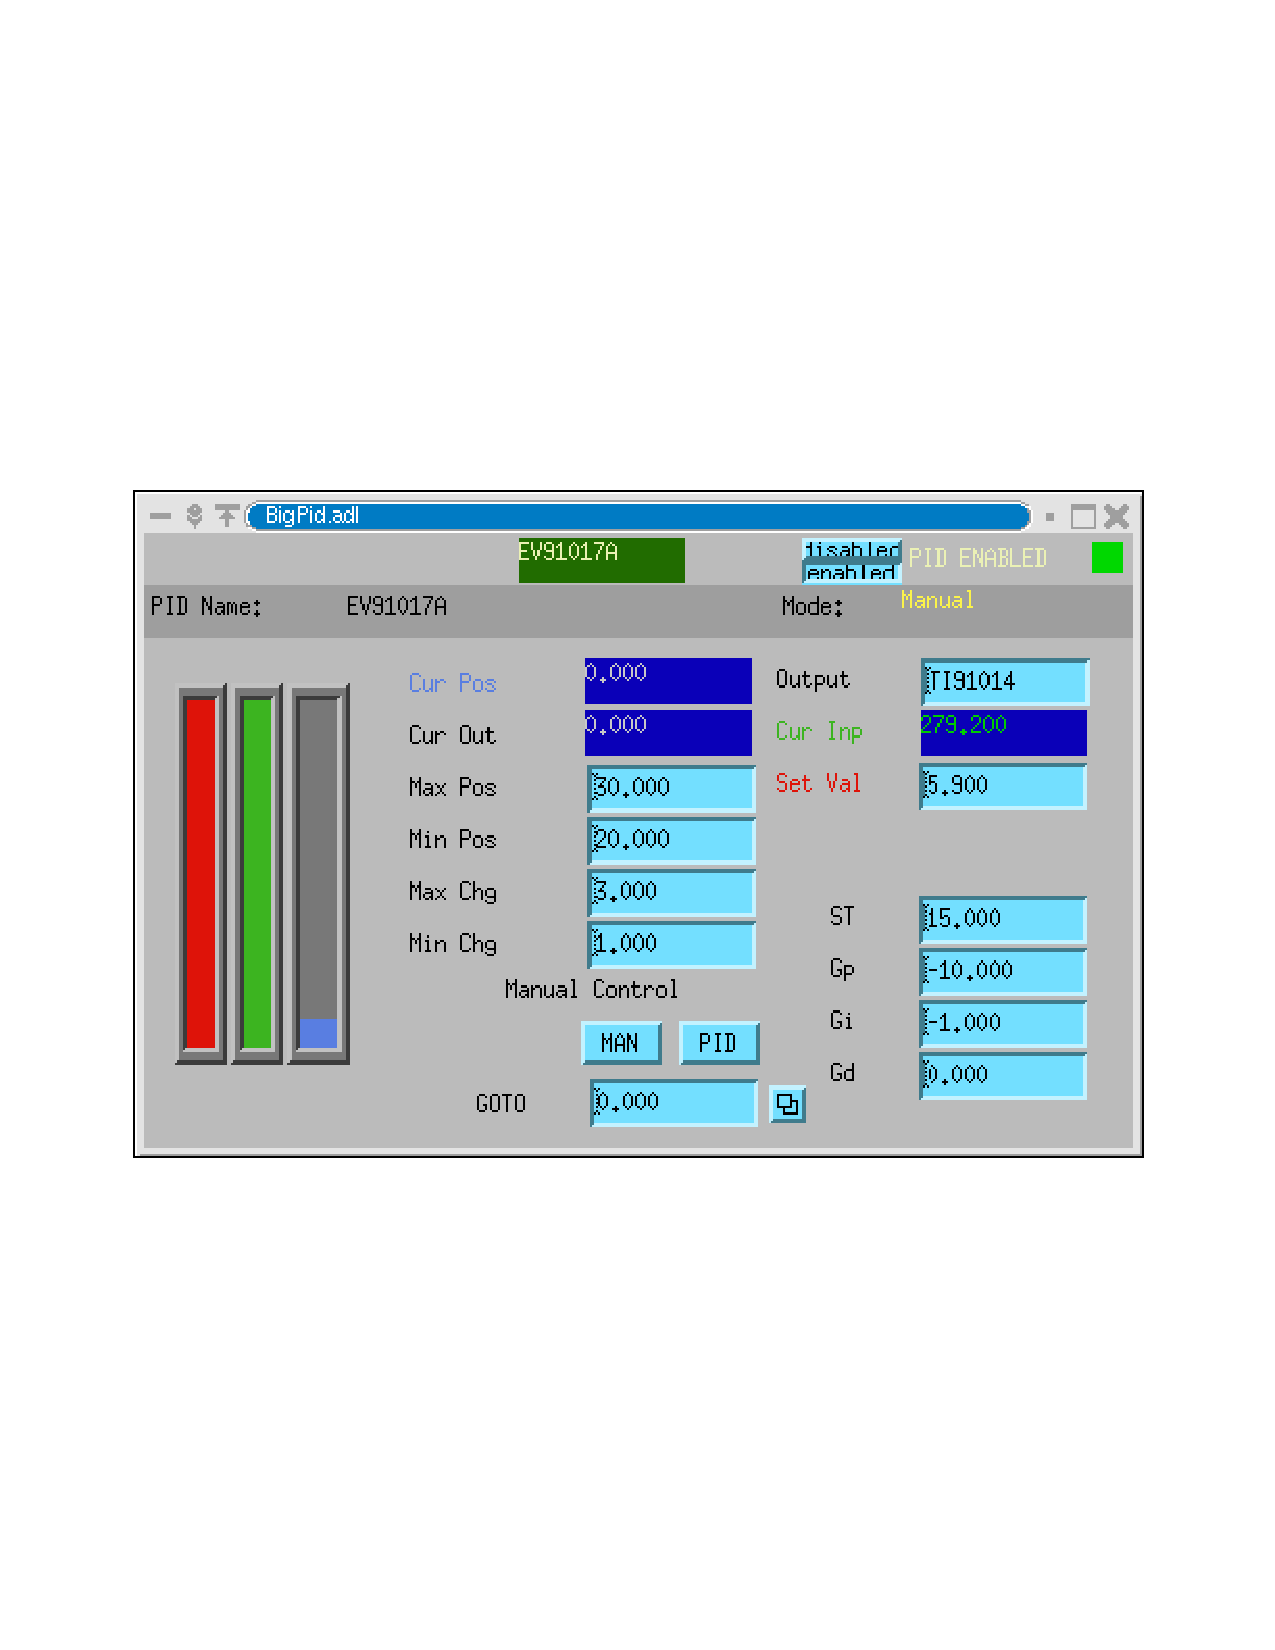
\includegraphics[width=3in]{ev91017a.pdf}
\caption{PID MEDM Screen - EV91017 Helium Supply Temperature Control}
\label{fig:ev17stc}
\end{figure}




\subparagraph{Detector HV}
The HV of all detectors is controlled from the SOS HV GUI. Nominal
settings for the PMT's are given in Table~\ref{tab:mol_hv}.  If
necessary, the M\o ller High Voltages can be controlled from the front
panel of the CAEN mainframe from which they are powered. This
mainframe is the only one in relay rack CHC15.
\begin{table}
\begin{center}
\caption{Nominal M\o ller Detector High Voltages and CAEN Power Supply Assignments\label{tab:mol_hv}}
\vspace{\baselineskip}
\begin{tabular}{|l|c|c|c|c|}
\hline
{}         & {}   & {}    & {}    & {}    \\
Detector   & Left & Left  & Right & Right \\
           & HV   & CAEN$\#$ & HV    & CAEN$\#$ \\
{}         & {}   & {}    & {}    & {}    \\ \hline
Pb Glass   & 1220* & 38   & 1310* & 39    \\
Hodo 01    & 1200  & 00   & 1220  & 05    \\
Hodo 02    & 1220  & 01   & 1190  & 06    \\
Hodo 03    & 1150  & 02   & 1120  & 07    \\
Hodo 04    & 1190  & 03   & 1100  & 08    \\
Hodo 05    & 1100  & 04   & 1120  & 09    \\
Hodo 06    & 1120  & 10   & 1200  & 15    \\
Hodo 07    & 1150  & 11   & 1100  & 16    \\
Hodo 08    & 1080  & 12   & 1270  & 17    \\
Hodo 09    & 1230  & 13   & 1100  & 18    \\
Hodo 10    & 1100  & 14   & 1180  & 19    \\
Hodo 11    & 1250  & 20   & 1150  & 25    \\
Hodo 12    & 1230  & 21   & 1200  & 26    \\
Hodo 13    & 1160  & 22   & 1150  & 27    \\
Hodo 14    & 1200  & 23   & 1180  & 28    \\
Hodo 15    & 1220  & 24   & 1170  & 29    \\
Hodo 16    & 1200  & 30   & 1150  & 35    \\
\hline
\end{tabular}
\end{center}
\end{table}
*{\it Note: The lead-glass voltages are beam energy dependent.}

\subparagraph{M\o ller IOCs Reference}

There is one IOC which support the M\o ller polarimeter device,
(iochc10 or {\it vmec10}). This IOC is on the accelerator network and
is managed by the accelerator group. It manages the superconducting
solenoid power supply and cryogenics system as well as the M\o ller
target and collimators.

The M\o ller target, collimators, solenoid power supply, and solenoid
cryogenics controls are all handled by vmec10 (also known as
iochc10). This IOC resides in the left hand side of a split-plane VME
crate in Hall C (behind the green wall, in the racks immediately to
the right as one enters the hall).  Its boot ROM looks like:

\texttt{\\
boot device          : ei \\
processor number     : 0 \\
host name            : opsrv \\
file name            : /cs/op/iocs/iochc10/vx/vxWorks \\
inet on ethernet (e) : 129.57.168.110:fffffc00 \\
inet on backplane (b): \\
host inet (h)        : 129.57.236.50 \\
gateway inet (g)     : 129.57.168.1 \\
user (u)             : vxwrks \\
ftp password (pw) (blank = use rsh): \\
flags (f)            : 0x0 \\
target name (tn)     : iochc10 \\
startup script (s)   : /cs/op/iocs/iochc10/startup \\
other (o)            : \\
}



%
\paragraph{Data acquisition}
The data acquisition reads out three Struck scaler modules at each
(possible) helicity transition. Scalers '1' and '2' are gated for '+'
and '-' helicity intervals as defined by the signal coming from
MCC. (For experiments using delayed helicity reporting the active
scaler will still be determined by the MCC signal, but this signal
does not necessarily indicate the instantaneous helicity state. The
actual state must be determined at analysis time.) Scaler '3' is gated
'on' during all helicity intervals, and should normally count the sum
of scalers '1' and '2'.

The CAMAC Crate is read out on an prescaled event by event basis
reading one ADC and one TDC module and two dual port memories. The ADC
and TDC provide diagnostic information about the lead glass shower
counters and the M\o ller coincidence timing. The memories provide
horizontal positioning information about the two M\o ller electrons in
front of the shower counters. This information is used to optimize the
quadrupole settings in order to center the 90$^{\circ}$ CM M\o ller
electrons on the lead glass. \\ \\ Data is taken using CODA2.5 running
on cdaql5. The DAQ can be started from the ``moller'' directory (in
the cdaq home directory) by invoking ``codamaster-moller.''

\paragraph{M\o ller Beam line tuning}

A thorough step-by-step procedure for tuning the beam through the
polarimeter has been worked out with the MCC operations group. Only
MCC operators may modify the settings of the M\o ller quadrupoles.
The procedure is available for your reference at
\htmladdnormallink{opsntsrv.acc.jlab.org/ops\_docs/MCC\_web\_interface/interface\_pages/operating\_procedures.asp}{opsntsrv.acc.jlab.org/ops\_docs/MCC\_web\_interface/interface\_pages/operating\_procedures.asp}. In addition, there is a companion 
document for Hall-C operators to follow. It is available in print form
in the counting room, or on the web at
\htmladdnormallink{Hall-C Moller Step-by-Step Guide}{http://www.jlab.org/Hall-C/document/manuals.html}.

The following is simply a coarse outline of the steps to be followed.
For actually tuning up the beamline and turning on the polarimeter,
you {\bf must} refer to the separate documents mentioned above. The
tuneup procedure should take no more than about 20 minutes if the beam
is already tuned to Hall~C.  The time required to ramp up the
superconducting solenoid is about 10 minutes.
\begin{enumerate}
        \item With all M\o ller magnets off MCC will
           center  the beam through the BPMs at 3C20 and 3C21  in both
           horizontal  and vertical  directions. 

        \item MCC will then turn on Q1, re-center the beam, then turn
	on Q2 and re-center the beam again. The required quad currents
	must be supplied by Hall~C.  (The M\o ller expert should have
	posted them in the logbook.)

        \item MCC will request that the Hall shift crew ramp up the
	M\o ller solenoid. We normally run it at 3~Tesla.

        \item With the solenoid and the two quadrupoles Q1, Q2, and Q3 on
              at nominal current, MCC will once again center the beam
              through the polarimeter and into the hall.

	\item If it is desired to take M\o ller measurements at beam currents
	      higher than $\approx$ 2 $\mu$ A it will be necessary to energize
	      the M\o ller raster system. See the documentation in
              \nolinkurl{\~cdaq/documents/beamline/Moller\_Raster\_Manual.txt}
\end{enumerate}




\begin{safetyen}{0}{0}
\infolevone{\subsection{Safety Information}}
%
% Information for the ESAD
%

The M\o ller Polarimeter integrates beamline elements (magnets and
vacuum systems) with particle detector systems. Typical hazards for
both types of systems are present.

\infolevone{\subsubsection{Hazards}}
\infoleveqnull{\subsection{Hazards}}

The are several specific hazards (potentially beyond those found in
the accelerator beamline) associated with the M\o ller Polarimeter.
These include:
\begin{enumerate}
\item{Radiation areas: These are potentially caused by use of the M\o ller using thick targets, at higher than normal currents, or at low energies.}
\item{Vacuum windows: There are thin vacuum windows at the ends of the M\o ller detector legs.}
\item{ODH : Inadvertent venting of the M\o ller cryostat could result in the creation of oxygen deficient areas in the beamline.}
\item{Electrical hazards: These exist in the vicinity of the magnet leads, as well as the detector high voltage.}
\item{Magnetic fields from the quadrupole and solenoid magnets.}
\end{enumerate}

\infolevone{\subsubsection{Mitigations}}
\infoleveqnull{\subsection{Mitigations}}

The special hazards associated with the Hall C M\o ller are mitigated as
described below.

\begin{enumerate}
        \item{Potential radiation areas are surveyed and posted before access to the hall is permitted
        after beam operations.}
        \item{The thin vacuum windows at the end of the M\o ller legs are mitigated by shields that prevent inadvertent
        punctures of the window. If work near the exit windows is required, hearing and eye protection is advised.}
        \item{ODH monitors are placed near the floor and ceiling in the Hall C beam tunnel due to the presence of cryogens
        in the M\o ller solenoid. The solenoid vent is also connected to permanent piping that runs into the hall proper.
        Finally, the area behind the beamline is marked ODH1, so that any work performed on the beam left side of the
        beamline requires a ``buddy.''}
        \item{Electrical hazards due to magnet leads are mitigated using Plexiglas shields where appropriate.
        The M\o ller detectors use standard SHV connectors.}
        \item{``Magnet on'' signs or blinking lights alert users to the presence of magnetic fields.}
\end{enumerate}

\noindent{}Additional safety information is available in the following documents:
\begin{list}{--}{\setlength{\itemsep}{-0.15cm}}
  \item EH\&S Manual~\cite{EHScebaf};
  \item PSS Description Document~\cite{PSScebaf}
  \item Accelerator Operations Directive~\cite{AODcebaf};
\end{list}

\infolevone{\subsubsection{Responsible Personnel}}
\infoleveqnull{\subsection{Responsible Personnel}}

Points of contact for the Hall C M\o ller Polarimeter are listed in the Tab.~\ref{tab:personnel_moller}.

\begin{namestab}{tab:personnel_moller}{M\o ller Polarimeter: authorized personnel}{%
   M\o ller Polarimeter points of contact.}
  \namestabheader{Hall C Physicists}
  \DaveGaskell{\em 1st Contact}
  \HowardFenker{\em 2nd Contact}
\end{namestab}
\end{safetyen}
}
